% !TeX root = ../main.tex

\chapter{Initial Booting of the PSC and Configuration of the EEPROM}
\label{chap:Initial Booting of the PSC and Configuration of the EEPROM}
\section{Overview}
This section will discuss the steps required for the first time booting a new PSC, and initializing the EEPROM.\\\\
\textbf{The EEPROM must be configured before many functions will work.}\\\\
It is important to note that once the EEPROM is configured, many parameters of the PSC will still provide inconsistent or invalid data until the QSPI values are initialized properly via the scripts outlined in \autoref{chap:Running the Calibration and Test Script}.

\subsection{Creating the SD Card}
First, a new SD card must be generated and installed in the PSC. We have been using Microcenter 32GB microSD cards, though other brands and sizes may (or may not) work.\\

\begin{enumerate}
	\item Download the BOOT.bin binaries from the git repository\\
	For convenience, the latest stable version of firmware is located in the test script repostiory outlined in \autoref{chap:Running the Calibration and Test Script}.\\\\
	Copy to your SD card this BOOT.bin
	
	\item Create and Save the NET.CNF file to the SD card\\
	A NET.CNF file is included in the repository as well, and can be used with no modifications so long as only one PSC is connected to the network at a time. Connecting more requires changing the static IP address set in this file for each PSC. 
	
	\item Eject the SD card, and install in the zPSC, it should now be ready to boot. 
	
	\item Turn on the PSC, it should boot, indicated by front panel LED D8 rapidly flashing. It may take 60 to 90 seconds for the PSC to connect to the network and ping, be patient.\\The PSC will take an extended amount of time to boot the RTOS if no ethernet cable is connected at all.  
\end{enumerate}

\subsection{Configuring the EEPROM}
Once the PSC has booted, we can proceed to writing the EEPROM configuration.\\
\begin{enumerate}
	\item Connect the micro-USB cable to the front panel port of the PSC, and identify which serial port it appears as on your terminal.\\
	You may need to do a directory list before and after plugging in, to see which serial device appears:\\
	\texttt{ls /dev}\\
	In this example, the PSC will appear as /dev/ttyUSB2.\\
	\begin{figure}[H]
		\centering
		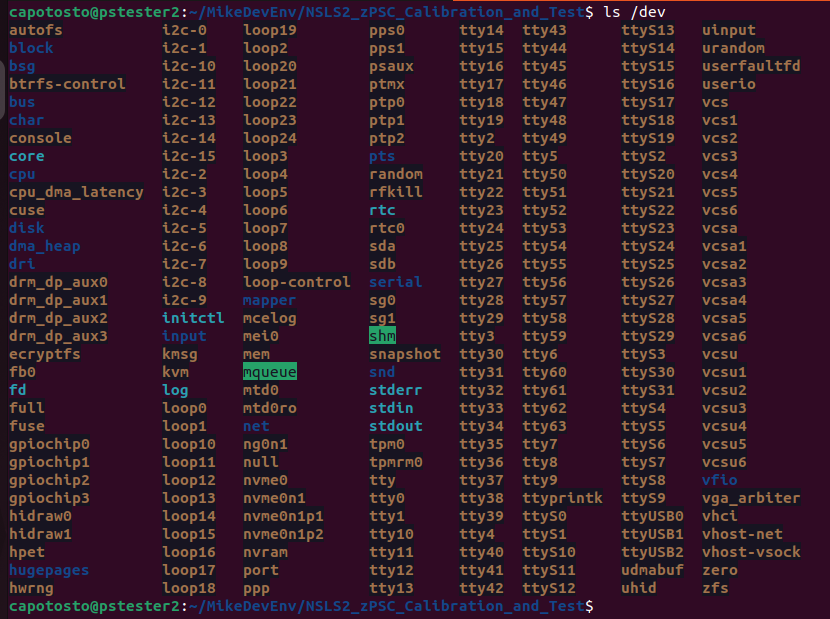
\includegraphics[width=\textwidth]{Python_Screenshots/ls_dev}
	\end{figure}
	\newpage
	\item Open Minicom using the port you determined: \texttt{minicom -D /dev/ttyUSB2}
		\begin{figure}[H]
			\centering
			\includegraphics[width=4in]{Python_Screenshots/EEPROM_Terminal}
		\end{figure}
	\item  Set Items B through E for a standard PSC, and F, G as needed.
		\begin{figure}[H]
			\centering
			\includegraphics[width=4in]{Python_Screenshots/minicom b}
			\caption{Setting B}
		\end{figure}
		\begin{figure}[H]
			\centering
			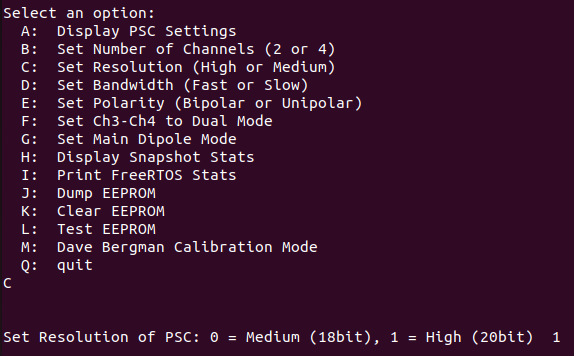
\includegraphics[width=4in]{Python_Screenshots/minicom c}
			\caption{Setting C}
		\end{figure}
		\begin{figure}[H]
			\centering
			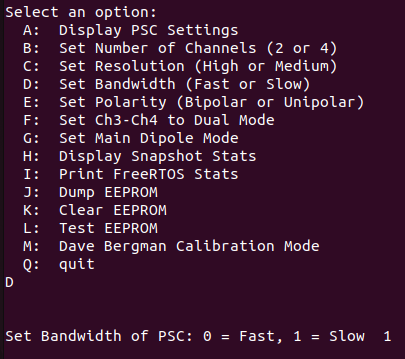
\includegraphics[width=4in]{Python_Screenshots/minicom d}
			\caption{Setting D}
		\end{figure}
		\begin{figure}[H]
			\centering
			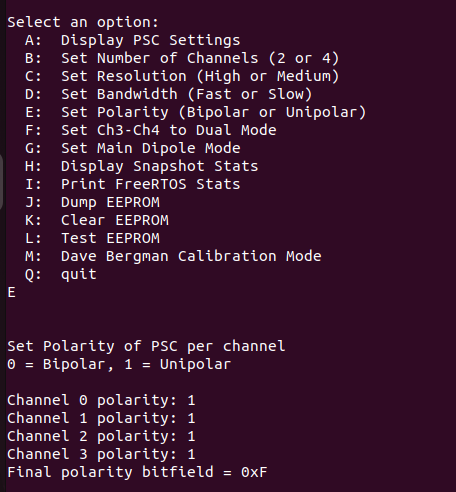
\includegraphics[width=4in]{Python_Screenshots/minicom e}
			\caption{Setting E}
		\end{figure}
	\newpage
	\item Verify the settings with Option A:
		\begin{figure}[H]
			\centering
			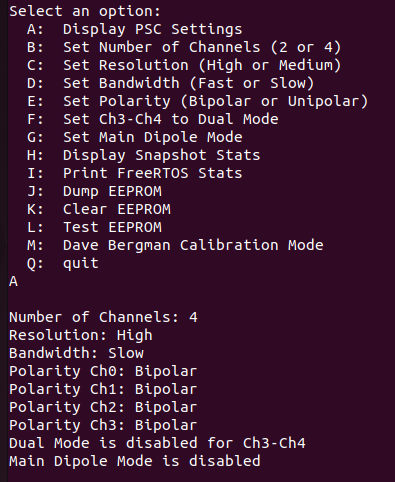
\includegraphics[width=4in]{Python_Screenshots/minicom a}
			\caption{Setting A}
		\end{figure}
	\item If satisfied, it is now safe to unplug the USB cable, no further action is necessary. To exit Minicom, press \texttt{ctrl+a}, release, press \texttt{x}, release, and finally press \texttt{<return>} for 'Yes' to exit.
\end{enumerate}